%chktex-file 46
%chktex-file 21
%chktex-file 3
%chktex-file 13
%chktex-file 8
%chktex-file 25

Concrete degradation is a crucial factor to consider in the risk assessment of radioactive waste disposal facilities due to its in potential structural and environmental failure. Over time, degradation processes such as carbonation can lower the alkalinity of concrete, which is essential for protecting the steel reinforcements within these structures from corrosion. The onset of corrosion can compromise the integrity of containment walls, potentially leading to breaches that could release radioactive materials into the environment. Properly accounting for these degradation pathways in risk assessments is essential for ensuring the containment's longevity and, hence, the protection of public health and the environment.
{{\textit{Add citation of the guy Ali knows}}}.

\subsection{Concrete degradation}
The two most critical degradation processes impacting concrete infrastructure in radioactive waste disposal are carbonation-induced corrosion and chloride-induced corrosion. This section provides a concise overview of both phenomena and presents their respective mathematical models.

\subsubsection{Carbonation-induced corrosion}\label{Carbonation_corrosion_Chpt}
The abundance of $CO_2$ increases the risk of carbonation-induced corrosion in concrete structures~\cite{TALUKDAR_part1,TALUKDAR_part2}. 
The interaction between concrete and atmospheric $CO_2$ causes the formation of calcium carbonate, a process known as carbonation, which reduces the concrete's alkalinity and makes the steel reinforcement in the concrete susceptible to corrosion, as presented by~\textcite{GLASSER2008226}.
Carbonation is quantified by measuring the depth from the concrete surface to where the alkalinity reaches a minimum allowable value. 
Once carbonation reaches the steel reinforcements, the corrosion propagation phase begins, accelerating the degradation of the concrete structure.
In this study, the carbonation depth, denoted as $x_c(t)$, is assessed using the methodology of~\textcite{Carb_eq_STEWART,Carb_eq_BASTIDASARTEAGA}.
Specifically, Eq.\ref{3:carbonation_depth} describes the increment in carbonation depth $\Delta x_c$ at time $t$, relative to the depth reached at time $t-\Delta \tau$, where $\Delta \tau$ denotes the selected evaluation interval in years, e.g., for a decade, $\Delta \tau = 10$.
\begin{equation}
    \label{3:carbonation_depth}
    \Delta x_c(t, \Delta \tau) = \sqrt{\frac{2 \ k_{site} \ C_{CO_2}(t) \ f_T^C(t) \ f_{RH}^C(t) \ (D_0^C)^{-n_d}}{a} \ \Delta \tau} \ \cdot \ \left( \frac{1}{\tau} \right)^{n_m} 
\end{equation}
In defining $\Delta x_c$, $\tau$ is an integer representing the number of $\Delta \tau$ intervals needed from the reference year to reach the evaluation year $t$, e.g., $t = 2020$ implies $\tau = 1$, $t = 2030$ implies $\tau = 2$, and so on.
The variable $k_{site}$ accounts for potentially higher $CO_2$ concentration values in industrial and urban areas; $C_{CO_2}$ is the time-dependent $CO_2$ concentration measured in \si{\kilogram\per\cubic\meter} is the $CO_2$ diffusion coefficient at reference time $\tau_0$, measured in \si{\square\meter\per\second}; $n_d$ is the diffusion coefficient aging factor; and $n_m$ is a factor accounting for exposure to microclimatic wetting and drying cycles, with a value of $0$ for sheltered outdoor environments, or $0.12$ for unsheltered outdoor. \\
The time-independent quantity $a$ is derived from Eq.\ref{eq_a}, where $\alpha_h$ is the degree of hydration, expressed as a function of the water-to-cement ratio $w / c$. The cement content $Ce$ is measured in \si{\kilogram\per\cubic\meter}, the calcium oxide fraction in cement $CaO$ is approximately 0.65, and the molar masses of $CO_2$ and $CaO$ are \SI{44}{\kilogram\per\mole} and \SI{56}{\kilogram\per\mole}, respectively.
\begin{equation}
    \left\{
    \begin{array}{ll}
    a = 0.75 \ Ce \ CaO \ \alpha_H \frac{M_{CO_2}}{M_{CaO}} \\
      \\
      \alpha_h = 1 - e^{-3.38 \frac{w}{c}}
    \end{array}
    \right.
    \label{eq_a}
\end{equation}
The time-dependent quantities $f_T^C$ and $f_{RH}^C$ allow the incorporation of climate variable effects, associated with climate change projections, into the carbonation depth evaluation, as presented in the analytical models by~\textcite{Carbonation_BASTIDASARTEAGA}. 
Specifically, $f_T^C$ represents the dynamic effect of temperature on carbonation, impacting the diffusion coefficient according to the Arrhenius Law~\cite{Carbonation_YOON}, as shown in Eq.\ref{3:ft}. Here, $E$ is the activation energy of the diffusion process, i.e.,
\SI{38.3}{\kilo\joule\per\mole}; $R$ is the gas constant, i.e., \SI{8.314}{\kilo\joule\per\mole\per\kelvin}; $T(t_0)$ is the reference temperature, i.e.,\SI{293}{\kelvin}; and $T(t)$ is the temperature in Kelvin at time $t$.
\begin{equation}
    \label{3:ft}
        f_T^C (t) = e^{\frac{E}{R} \left[ \frac{1}{T_0} - \frac{1}{T(t)} \right]}
\end{equation}
The effect of relative humidity (RH) has been extensively studied. Research by~\textcite{f_rh_Al-Khaiat} suggests that RH levels below 30\% do not significantly impact carbonation depth, whereas~\textcite{f_rh_BARY} indicates that RH levels above 50\% have a significant influence. For this study, the analytical model chosen to describe the RH effect over time on the diffusion coefficient is the one proposed by~\textcite{Carbonation_BASTIDASARTEAGA}, detailed in Eq.\ref{3:frh}.
\begin{equation}
    \left\{
    \begin{array}{ll}
    0 & if \ RH \leq 0.25\\
    \left[\frac{1-RH(t)^\beta}{1-RH_0^\beta} \right]^\alpha & otherwise
    \end{array}
    \right.
    \label{3:frh}
\end{equation}
Here, $RH_0$ is the reference value for RH, while $\alpha$ and $\beta$ are independent parameters of exposure conditions. In this case study, the reference RH is set to 0.65, $\alpha$ is 5, and $\beta$ is 2.5.

\subsubsection{Chloride-induced corrosion}\label{Chloride_corrosion_Chpt}
The penetration and movement of chloride ions into concrete structures involve the electrochemical dissolution of iron, leading to the degradation of concrete barriers.
Chloride ingress into concrete is typically described using a diffusion model, which is a single mass transport equation for chloride ion transport.
In this study, a time-dependent model is applied, incorporating the chloride diffusion coefficient to estimate chloride concentration over time. The chloride concentration at a depth $z$ and time $t$ is described by Eq.\ref{eq:chloride_corrosion}.
\begin{equation}
    \label{eq:chloride_corrosion}
    C(z, t) = C_0^{Cl} \left[ 1-erf \left(\frac{z}{2\sqrt{k_e \ k_t \ k_c \ f_T^{Cl}(t) \ f_{RH}^{Cl}(t) \ D_0^{Cl} \ \omega \tau}} \right) \right]
\end{equation}
Here, $C_0^{Cl}$ represents the chloride concentration at the boundary; for atmospheric areas remote from coasts, $C_0^{Cl}$ is typically around \SI{1.15}{\kilogram\per\cubic\meter}, whereas, in coastal or tidal areas, the chloride concentration at the surface is significantly higher. $D_0^{Cl}$ is the reference chloride diffusion coefficient; $k_e$ is the environmental coefficient; $k_t$ is the test method factor, and $k_c$ is the curing factor. 
Similar to carbonation, there are two time-dependent quantities that account for the effects of climate change projections on temperature and relative humidity: $f_{T}^{Cl}$ and $f_{RH}^{Cl}$.
\begin{equation}
    \label{eq_f_rh_cl}
    f_{RH}^{Cl}(t) = \left[ 1 + \frac{(1-RH(t))^4}{(1-RH_0)^4} \right]^{-1}
\end{equation}
The temperature effect is consistent with that defined for carbonation in Eq.\ref{3:ft}, thus $f_T^C = f_T^{Cl}$. The effect of RH is expressed in the work of~\textcite{f_RH_ClELHASSAN} as shown in Eq.\ref{eq_f_rh_cl}.

\subsection{eBN for concrete degradation}
The eBN framework is the selected approach to perform risk analysis for concrete degradation considering climate change. Climate change data are taken from the catalogue produced by~\textcite{Copernicus_Climate_Change} and includes three main projection scenarios refered to three different shared socioeconomic pathway (SSP), namely \textit{ssp1}, \textit{ssp2}, and \textit{ssp5}. These pathways provide different pathways of the future climate forcing and account for variations in temperature, $CO_2$ concentration, and relative humidity from 2020 to 2100. 
In this study the eBN integrates the two degradation models presented in~\ref{Carbonation_corrosion_Chpt}, and in~\ref{Chloride_corrosion_Chpt} and is structured to capture the probabilistic dependencies considering epistemic and aleatoric uncertainties, between climate conditions of temperature, relative humidity, and CO₂ concentration, material properties, such as diffusion coefficients, water-to-cement ratio, and the final state of the system, through the carbonation and chloride effect on concrete.

The following sections details the eBN structure, the probabilistic modeling of input variables, and its application to the case study of a radioactive waste disposal concrete degradation. Initially, the carbonation-induced and chloride-induced corrosion models are examined separately to enhance clarity and comprehensibility. Subsequently, the complete eBN framework, integrating both degradation mechanisms, is presented.

\subsubsection{eBN -- Carbonation-induced corrosion model}\label{ebn_carbonation_section}
The eBN representing the carbonation process, illustrated in Fig.~\ref{carbonation_ebn}, includes two primary discrete root nodes. The first is the node \textit{t}, which denotes the selected time slice aligned with climate change projections; it consists of nine equally probable states, corresponding to the decades from 2020 to 2100. The second node, \textit{proj}, represents the climate change scenario, with three equally likely states, each associated with a distinct projection.
\begin{figure}[H]
    \centering
    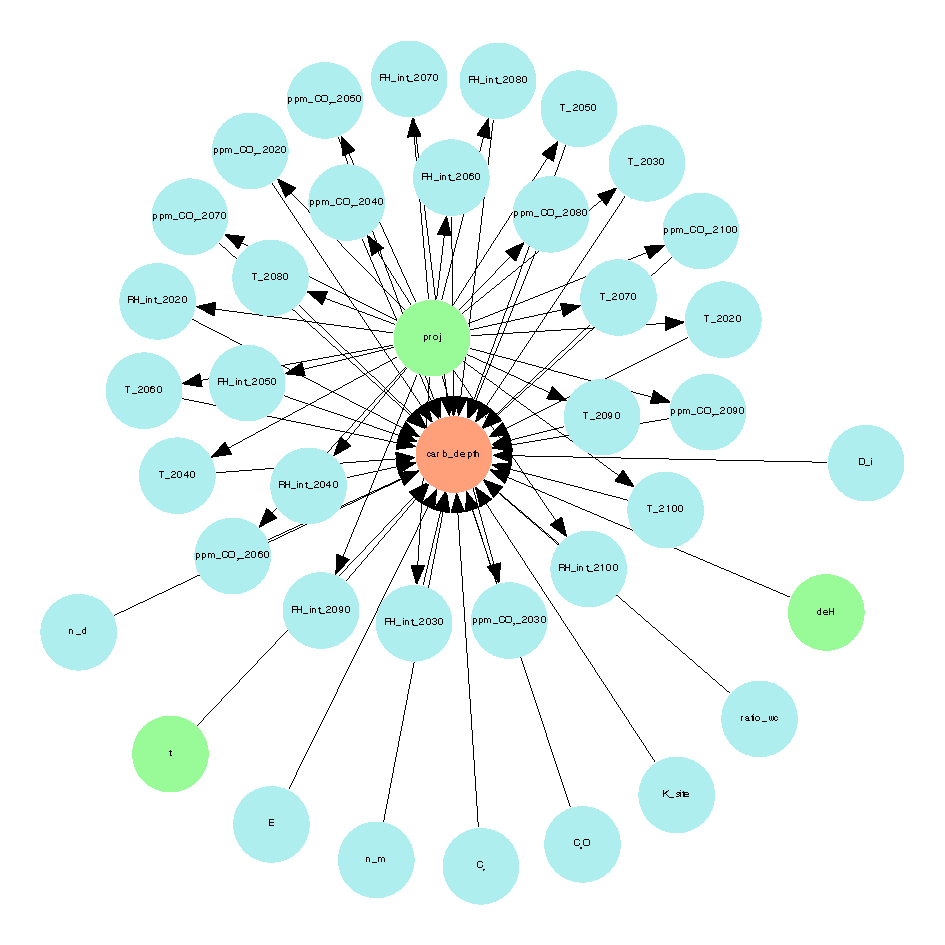
\includegraphics[width=\linewidth]{imgs/pdfs/8_carb_ebn.pdf}
    \caption{Carbonation phenomenon eBN with precise nodes}\label{carbonation_ebn}
\end{figure}
A third discrete root node, \textit{DeH}, is also shown in Fig.~\ref{carbonation_ebn}. This node represents a system designed to control and reduce the RH below a threshold. Specifically, whenever RH exceeds 0.25, the node enforces a reduction to 0.2. These values were selected based on the influence of RH on the carbonation model, as illustrated in Fig.~\ref{carbonation_depth vs RH}.
\begin{figure}[H]
    \centering
    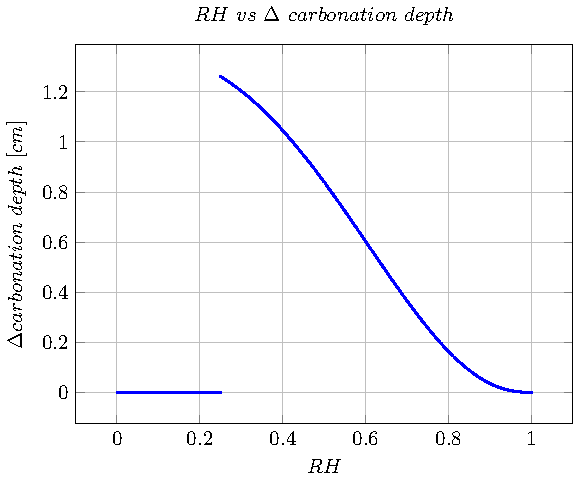
\includegraphics[width=\linewidth]{imgs/pdfs/10_RH_carb.pdf}
    \caption{RH effect on carbonation depth}\label{carbonation_depth vs RH}
\end{figure}
The \textit{DeH} node is modelled as a Boolean variable with two states: failed ($P_{F} = 10^{-4}$) and working ($P_{W} = 1 - 10^{-4}$). \\
In addition, eight continuous root nodes are introduced to account for aleatoric uncertainties in the parameters $n_d$, $n_m$, $E$, $k_{site}$, water-to-cement ratio ($w/c$), $C_e$, $CaO$, and $D_0^C$. Their CPTs are provided in Table~\ref{continuous_root_node_ebn_carb}.
\begin{table}[hbt!]
    \begin{center}
        \caption{Continuous root node distribution of the eBN in Fig.\ref{carbonation_ebn}}\label{continuous_root_node_ebn_carb}
        \begin{tabular}{P{1.6cm}P{2.1cm}P{6cm}}
            \textbf{Quantity} & \textbf{Node Name} & \textbf{Distribution} \\
            \midrule
            $n_d$       & $n \_ d$          & $Trunc(N(0.24;2.88e^{-2}); 0, \infty)$ \\
            $n_m$       & $n \_ m$          & $Trunc(N(0.12;1.2e^{-2}); 0, \infty)$\\
            $E$         & $E$               & $Uniform(34.853;41.747)$ \\
            $k_{site}$  & $k \_ site$       & $Trunc(N(1.15;1.15e^{-2}); 0, \infty)$ \\
            $w / c$     & $ratio \_ w/c$    & $Trunc(LogN(-0.69; 0.05); 0, 1)$ \\
            $Ce$        & $C_e$             & $Trunc(N(300;30); 0, \infty)$ \\
            $CaO$       & $C_aO$            & $Uniform(0.585; 0.715)$ \\
            $D_0^C$     & $D \_ i$          & $Trunc(N(2.2e^{-4};1.5e^{-5}); 0, \infty)$ \\
        \end{tabular}
    \end{center}
\end{table}
The carbonation process is governed by the model in Eq.~\ref{3:carbonation_depth}, which explicitly depends on temperature, $CO_2$ concentration, and RH. These variables are characterized through climate change projections.he model is dynamic in nature, as its output corresponds to the increment in carbonation depth accumulated over the decade ending in the year under consideration. Therefore, to evaluate the total carbonation depth, one must consider the cumulative sum of increments from all preceding decades.
To address this dynamic behavior, the authors introduced decade-specific nodes for temperature, $CO_2$ concentration (in ppm), and relative humidity deviation (in percentage). Examples include $T\_ {2020}$, $T\_ {2030}$, and so on up to $T\_ {2100}$, as shown in Fig.~\ref{carbonation_ebn}. These nodes are all modeled as children of the \textit{proj} node, with distributions detailed in Tables~\ref{Climate_Change_Tnode_dists},~\ref{Climate_Change_RHnode_dists}, and~\ref{Climate_Change_CO2node_dists}.
This structure supports the definition of the functional node \textit{carb\_depth}, which is a child of all temperature, $CO_2$, and RH nodes, as well as of \textit{proj}, \textit{DeH}, and the time slice node \textit{t}. For each time step, a dedicated model computes the incremental carbonation depth by summing contributions from previous decades. If the resulting total exceeds the threshold of 3 cm, the system transitions to a failure state. 
In the carbonation model, the inputs from the $ratio\_w/c$ node and all the RH percentage change nodes are modified before being passed to the computational component. Specifically, the $ratio\_w/c$ samples are scaled by a factor of 0.1 and then shifted by +0.5, while the RH percentage change samples are randomly assigned as either positive or negative deviations from the reference RH.
Further implementation details for the \textit{carb\_depth} node are available in the associated code.
\begin{table}[H]
    \begin{center}
    \caption{Temperature nodes CPTs for the precise eBN of Fig.\ref{carbonation_ebn}. Temperatures are measured in $K$}\label{Climate_Change_Tnode_dists}
        \begin{tabular}{P{2.5cm}P{8cm}}
            \toprule
            \textbf{Node} & \textbf{CPT} \\
            \midrule
            $T \_ 2020$ & 
                \begin{tabular}{P{2cm}P{5cm}}
                    \textbf{proj} & \textbf{distribution} \\
                    \midrule
                    \:ssp1 & $Trunc(N(283.9; 0.85); 0, \infty)$ \\
                    \:ssp2 & $Trunc(N(284.1; 0.85); 0, \infty)$ \\
                    \:ssp5 & $Trunc(N(283.9; 0.85); 0, \infty)$ \\
                \end{tabular}
            \\
            \midrule
            $T \_ 2030$ & 
                \begin{tabular}{P{2cm}P{5cm}}
                    \textbf{proj} & \textbf{distribution} \\
                    \midrule
                    \:ssp1 & $Trunc(N(284.2; 0.85); 0, \infty)$ \\
                    \:ssp2 & $Trunc(N(284.2; 0.85); 0, \infty)$ \\
                    \:ssp5 & $Trunc(N(284.3; 1.13); 0, \infty)$ \\
                \end{tabular}
            \\
            \midrule
            $T \_ 2040$ & 
                \begin{tabular}{P{2cm}P{5cm}}
                    \textbf{proj} & \textbf{distribution} \\
                    \midrule
                    \:ssp1 & $Trunc(N(284.2; 0.85); 0, \infty)$ \\
                    \:ssp2 & $Trunc(N(284.6; 0.85); 0, \infty)$ \\
                    \:ssp5 & $Trunc(N(284.9; 1.14); 0, \infty)$ \\
                \end{tabular}
            \\
            \midrule
            $T \_ 2050$ & 
                \begin{tabular}{P{2cm}P{5cm}}
                    \textbf{proj} & \textbf{distribution} \\
                    \midrule
                    \:ssp1 & $Trunc(N(284.5; 0.85); 0, \infty)$ \\
                    \:ssp2 & $Trunc(N(284.8; 1.14); 0, \infty)$ \\
                    \:ssp5 & $Trunc(N(285.4; 1.14); 0, \infty)$ \\
                \end{tabular}
            \\
            \midrule
            $T \_ 2060$ & 
                \begin{tabular}{P{2cm}P{5cm}}
                    \textbf{proj} & \textbf{distribution} \\
                    \midrule
                    \:ssp1 & $Trunc(N(284.7; 1.13); 0, \infty)$ \\
                    \:ssp2 & $Trunc(N(285.1; 0.85); 0, \infty)$ \\
                    \:ssp5 & $Trunc(N(285.9; 1.14); 0, \infty)$ \\
                \end{tabular}
            \\
            \midrule
            $T \_ 2070$ & 
                \begin{tabular}{P{2cm}P{5cm}}
                    \textbf{proj} & \textbf{distribution} \\
                    \midrule
                    \:ssp1 & $Trunc(N(284.7; 1.13); 0, \infty)$ \\
                    \:ssp2 & $Trunc(N(285.2; 1.14); 0, \infty)$ \\
                    \:ssp5 & $Trunc(N(286.5; 1.15); 0, \infty)$ \\
                \end{tabular}
            \\
            \midrule
            $T \_ 2080$ & 
                \begin{tabular}{P{2cm}P{5cm}}
                    \textbf{proj} & \textbf{distribution} \\
                    \midrule
                    \:ssp1 & $Trunc(N(285.0; 1.14); 0, \infty)$ \\
                    \:ssp2 & $Trunc(N(285.4; 1.14); 0, \infty)$ \\
                    \:ssp5 & $Trunc(N(287.4; 1.44); 0, \infty)$ \\
                \end{tabular}
            \\
            \midrule
            $T \_ 2090$ & 
                \begin{tabular}{P{2cm}P{5cm}}
                    \textbf{proj} & \textbf{distribution} \\
                    \midrule
                    \:ssp1 & $Trunc(N(284.8; 1.42); 0, \infty)$ \\
                    \:ssp2 & $Trunc(N(286.7; 1.14); 0, \infty)$ \\
                    \:ssp5 & $Trunc(N(288.1; 1.44); 0, \infty)$ \\
                \end{tabular}
            \\
            \midrule
            $T \_ 2100$ & 
                \begin{tabular}{P{2cm}P{5cm}}
                    \textbf{proj} & \textbf{distribution} \\
                    \midrule
                    \:ssp1 & $Trunc(N(283.7; 1.42); 0, \infty)$ \\
                    \:ssp2 & $Trunc(N(286.0; 1.14); 0, \infty)$ \\
                    \:ssp5 & $Trunc(N(288.9; 1.45); 0, \infty)$ \\
                \end{tabular}
        \end{tabular}
    \end{center}
\end{table}

\begin{table}[H]
    \begin{center}
        \caption{RH nodes CPTs for the precise eBN of Fig.\ref{carbonation_ebn}. RH is expressed in percentage of deviation wth respect to the reference value $RH_{ref}$ = 0.65}\label{Climate_Change_RHnode_dists}
        \begin{tabular}{P{2.5cm}P{8cm}}
            \toprule
            \textbf{Node} & \textbf{CPT} \\
            \midrule
            $RH \_ int \_ 2020$ & 
                \begin{tabular}{P{2cm}P{5cm}}
                    \textbf{proj} & \textbf{distribution} \\
                    \midrule
                    \:ssp1 & $Trunc(N(9.35e^{-2}; 5.66e^{-2}); 0, 1)$ \\
                    \:ssp2 & $Trunc(N(8.48e^{-2}; 6.42e^{-2}); 0, 1)$ \\
                    \:ssp5 & $Trunc(N(8.19e^{-2}; 5.00e^{-2}); 0, 1)$ \\
                \end{tabular}
            \\
            \midrule
            $RH \_ int \_ 2030$ & 
                \begin{tabular}{P{2cm}P{5cm}}
                    \textbf{proj} & \textbf{distribution} \\
                    \midrule
                    \:ssp1 & $Trunc(N(9.52e^{-2}; 5.20e^{-2}); 0, 1)$ \\
                    \:ssp2 & $Trunc(N(9.18e^{-2}; 5.42e^{-2}); 0, 1)$ \\
                    \:ssp5 & $Trunc(N(1.11e^{-1}; 5.83e^{-2}); 0, 1)$ \\
                \end{tabular}
            \\
            \midrule
            $RH \_ int \_ 2040$ & 
                \begin{tabular}{P{2cm}P{5cm}}
                    \textbf{proj} & \textbf{distribution} \\
                    \midrule
                    \:ssp1 & $Trunc(N(1.01e^{-1}; 5.67e^{-2}); 0, 1)$ \\
                    \:ssp2 & $Trunc(N(1.12e^{-1}; 6.61e^{-2}); 0, 1)$ \\
                    \:ssp5 & $Trunc(N(1.44e^{-1}; 7.07e^{-2}); 0, 1)$ \\
                \end{tabular}
            \\
            \midrule
            $RH \_ int \_ 2050$ & 
                \begin{tabular}{P{2cm}P{5cm}}
                    \textbf{proj} & \textbf{distribution} \\
                    \midrule
                    \:ssp1 & $Trunc(N(1.16e^{-1}; 6.56e^{-2}); 0, 1)$ \\
                    \:ssp2 & $Trunc(N(1.34e^{-1}; 6.63e^{-2}); 0, 1)$ \\
                    \:ssp5 & $Trunc(N(1.66e^{-1}; 6.73e^{-2}); 0, 1)$ \\
                \end{tabular}
            \\
            \midrule
            $RH \_ int \_ 2060$ & 
                \begin{tabular}{P{2cm}P{5cm}}
                    \textbf{proj} & \textbf{distribution} \\
                    \midrule
                    \:ssp1 & $Trunc(N(1.27e^{-1}; 6.63e^{-2}); 0, 1)$ \\
                    \:ssp2 & $Trunc(N(1.50e^{-1}; 7.39e^{-2}); 0, 1)$ \\
                    \:ssp5 & $Trunc(N(1.90e^{-1}; 7.26e^{-2}); 0, 1)$ \\
                \end{tabular}
            \\
            \midrule
            $RH \_ int \_ 2070$ & 
                \begin{tabular}{P{2cm}P{5cm}}
                    \textbf{proj} & \textbf{distribution} \\
                    \midrule
                    \:ssp1 & $Trunc(N(1.25e^{-1}; 6.80e^{-2}); 0, 1)$ \\
                    \:ssp2 & $Trunc(N(1.60e^{-1}; 8.14e^{-2}); 0, 1)$ \\
                    \:ssp5 & $Trunc(N(2.30e^{-1}; 8.92e^{-2}); 0, 1)$ \\   
                \end{tabular}
            \\
            \midrule
            $RH \_ int \_ 2080$ & 
                \begin{tabular}{P{2cm}P{5cm}}
                    \textbf{proj} & \textbf{distribution} \\
                    \midrule
                    \:ssp1 & $Trunc(N(1.42e^{-1}; 7.54e^{-2}); 0, 1)$ \\
                    \:ssp2 & $Trunc(N(1.71e^{-1}; 7.88e^{-2}); 0, 1)$ \\
                    \:ssp5 & $Trunc(N(2.95e^{-1}; 1.91e^{-1}); 0, 1)$ \\   
                \end{tabular}
            \\
            \midrule
            $RH \_ int \_ 2090$ & 
                \begin{tabular}{P{2cm}P{5cm}}
                    \textbf{proj} & \textbf{distribution} \\
                    \midrule
                    \:ssp1 & $Trunc(N(1.41e^{-1}; 8.12e^{-2}); 0, 1)$ \\
                    \:ssp2 & $Trunc(N(1.79e^{-1}; 8.25e^{-2}); 0, 1)$ \\
                    \:ssp5 & $Trunc(N(3.28e^{-1}; 1.24e^{-1}); 0, 1)$ \\
                \end{tabular}
            \\
            \midrule
            $RH \_ int \_ 2100$ & 
                \begin{tabular}{P{2cm}P{5cm}}
                    \textbf{proj} & \textbf{distribution} \\
                    \midrule
                    \:ssp1 & $Trunc(N(1.34e^{-1}; 8.97e^{-2}); 0, 1)$ \\
                    \:ssp2 & $Trunc(N(1.96e^{-1}; 8.64e^{-2}); 0, 1)$ \\
                    \:ssp5 & $Trunc(N(3.85e^{-1}; 1.43e^{-1}); 0, 1)$ \\
                \end{tabular}
        \end{tabular}
    \end{center}
\end{table}

\begin{table}[H]
    \begin{center}
    \caption{$CO_2$ concentration nodes CPTs for the precise eBN of Fig.\ref{carbonation_ebn}. $CO_2$ concentrations are measured in $ppm$}\label{Climate_Change_CO2node_dists}
        \begin{tabular}{P{2.7cm}P{8cm}}
            \toprule
            \textbf{Node} & \textbf{CPT} \\
            \midrule
            $ppm \_CO_2 \_ 2020$ & 
                \begin{tabular}{P{2cm}P{5cm}}
                    \textbf{proj} & \textbf{distribution} \\
                    \midrule
                    \:ssp1 & $412.5$ \\
                    \:ssp2 & $412.5$ \\
                    \:ssp5 & $412.5$ \\
                \end{tabular}
            \\
            \midrule
            $ppm \_CO_2 \_ 2030$ & 
                \begin{tabular}{P{2cm}P{5cm}}
                    \textbf{proj} & \textbf{distribution} \\
                    \midrule
                    \:ssp1 & $Trunc(N(430.8; 6.89); 0)$ \\
                    \:ssp2 & $Trunc(N(435.0; 7.83); 0)$ \\
                    \:ssp5 & $Trunc(N(448.8; 9.87); 0)$ \\
                \end{tabular}
            \\
            \midrule
            $ppm \_CO_2 \_ 2040$ & 
                \begin{tabular}{P{2cm}P{5cm}}
                    \textbf{proj} & \textbf{distribution} \\
                    \midrule
                    \:ssp1 & $Trunc(N(440.2; 6.89); 0)$ \\
                    \:ssp2 & $Trunc(N(460.8; 7.37); 0)$ \\
                    \:ssp5 & $Trunc(N(489.4; 8.80); 0)$ \\
                \end{tabular}
            \\
            \midrule
            $ppm \_CO_2 \_ 2050$ & 
                \begin{tabular}{P{2cm}P{5cm}}
                    \textbf{proj} & \textbf{distribution} \\
                    \midrule
                    \:ssp1 & $Trunc(N(442.7; 7.52); 0)$ \\
                    \:ssp2 & $Trunc(N(486.5; 7.30); 0)$ \\
                    \:ssp5 & $Trunc(N(540.5; 10.27); 0)$ \\
                \end{tabular}
            \\
            \midrule
            $ppm \_CO_2 \_ 2060$ & 
                \begin{tabular}{P{2cm}P{5cm}}
                    \textbf{proj} & \textbf{distribution} \\
                    \midrule
                    \:ssp1 & $Trunc(N(441.7; 4.41); 0)$ \\
                    \:ssp2 & $Trunc(N(508.9; 8.14); 0)$ \\
                    \:ssp5 & $Trunc(N(603.5; 9.05); 0)$ \\
                \end{tabular}
            \\
            \midrule
            $ppm \_CO_2 \_ 2070$ & 
                \begin{tabular}{P{2cm}P{5cm}}
                    \textbf{proj} & \textbf{distribution} \\
                    \midrule
                    \:ssp1 & $Trunc(N(437.5; 3.50); 0)$ \\
                    \:ssp2 & $Trunc(N(524.3; 7.34); 0)$ \\
                    \:ssp5 & $Trunc(N(677.1; 8.80); 0)$ \\
                \end{tabular}
            \\
            \midrule
            $ppm \_CO_2 \_ 2080$ & 
                \begin{tabular}{P{2cm}P{5cm}}
                    \textbf{proj} & \textbf{distribution} \\
                    \midrule
                    \:ssp1 & $Trunc(N(431.6; 3.88); 0)$ \\
                    \:ssp2 & $Trunc(N(531.1; 6.37); 0)$ \\
                    \:ssp5 & $Trunc(N(758.2; 9.86); 0)$ \\
                \end{tabular}
            \\
            \midrule
            $ppm \_CO_2 \_ 2090$ & 
                \begin{tabular}{P{2cm}P{5cm}}
                    \textbf{proj} & \textbf{distribution} \\
                    \midrule
                    \:ssp1 & $Trunc(N(426.0; 4.26); 0)$ \\
                    \:ssp2 & $Trunc(N(533.7; 5.34); 0)$ \\
                    \:ssp5 & $Trunc(N(844.8; 10.13); 0)$ \\
                \end{tabular}
            \\
            \midrule
            $ppm \_CO_2 \_ 2100$ & 
                \begin{tabular}{P{2cm}P{5cm}}
                    \textbf{proj} & \textbf{distribution} \\
                    \midrule
                    \:ssp1 & $Trunc(N(420.9; 4.63); 0)$ \\
                    \:ssp2 & $Trunc(N(538.4; 4.30); 0)$ \\
                    \:ssp5 & $Trunc(N(935.9; 9.36); 0)$ \\
                \end{tabular}
        \end{tabular}
    \end{center}
\end{table}

\subsubsection{eBN -- Chloride-induced corrosion model}\label{ebn_chloride_section}
The chloride-induced corrosion process is represented by the eBN depicted in Fig.~\ref{chloride_ebn}. This model includes some of the same continuous nodes as the corrosion process eBN, specifically for temperature, $CO_2$ concentration, RH percentage change, and the activation energy $E$. It also shares the  discrete nodes \textit{proj}, \textit{t} and \textit{DeH}. The effect of relative humidity on the chloride penetration is shown in Fig.~\ref{RH vs chloride depth}
\begin{figure}[H]
    \centering
    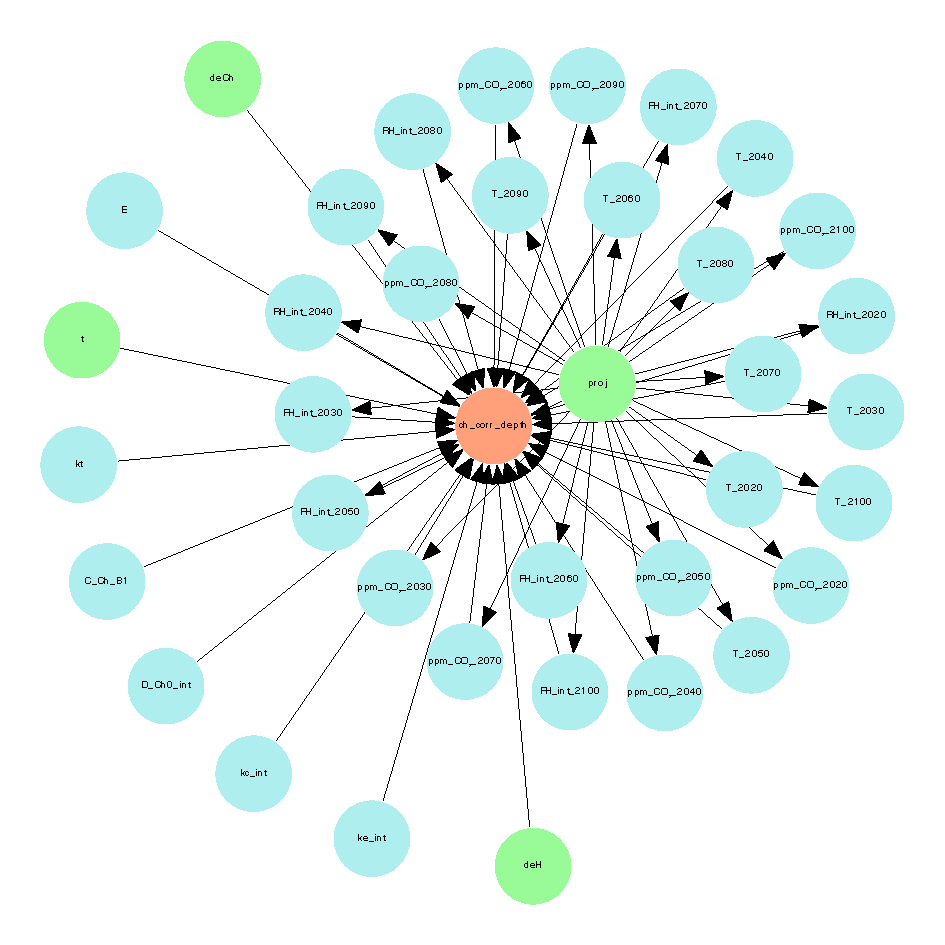
\includegraphics[width=\linewidth]{imgs/pdfs/9_chloride_ebn.pdf}
    \caption{Chloride-induced corrosion phenomenon eBN with precise nodes}\label{chloride_ebn}
\end{figure}
\begin{figure}[H]
    \centering
    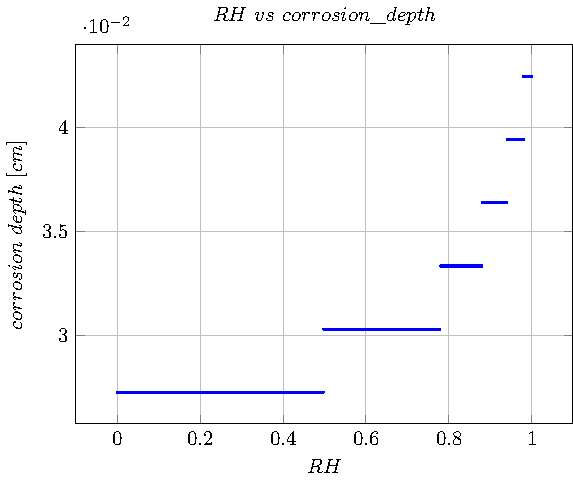
\includegraphics[width=\linewidth]{imgs/pdfs/11_RH_corr.pdf}
    \caption{RH effect on chloride depth}\label{RH vs chloride depth}
\end{figure}
\begin{figure}[H]
    \centering
    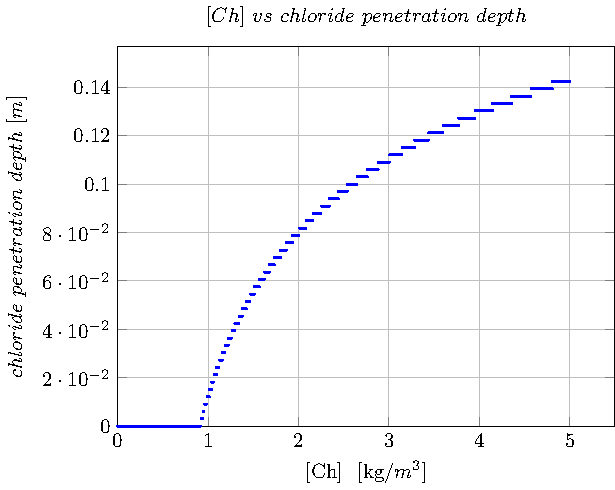
\includegraphics[width=\linewidth]{imgs/pdfs/11_Chloride_corr.pdf}
    \caption{Chloride concentration at system boundary effect on chloride depth}\label{Chloride vs corrosion depth}
\end{figure}

In addition to these, the model introduces a discrete root node, \textit{DeCh}, representing a chloride mitigation system that reduces the boundary chloride concentration, $C_0^{Cl}$, when it exceeds a critical level. The effect of the boundary chloride concentration on the model is shown in Fig.~\ref{Chloride vs corrosion depth}. $DeCh$ node is modelled as a Boolean variable with states \textit{working} and \textit{failed}, with assigned probabilities $P_W = 1 - 10^{-4}$ and $P_F = 10^{-4}$, respectively. When operational, the system lowers $C_0^{Cl}$ from values above 0.9 to 0.7. \\
Five continuous root nodes are also included to represent aleatoric uncertainties in the parameters $k_t$, $k_c$, $k_e$, $C_0^{Cl}$, and the reference diffusion coefficient $D_0^{Cl}$. Their CPTs are detailed in Table~\ref{continuous_root_node_ebn_ch}.

\begin{table}[hbt!]
    \begin{center}
        \caption{Continuous root node distribution of the eBN in Fig.\ref{chloride_ebn}}\label{continuous_root_node_ebn_ch}
        \begin{tabular}{P{1.6cm}P{2.1cm}P{6cm}}
            \textbf{Quantity} & \textbf{Node Name} & \textbf{Distribution} \\
            \midrule
            $k_t$       & $kt \_ int$      & $Trunc(N(0.832;2.4e^{-2}); 0, \infty)$ \\
            $k_e$       & $ke \_ int$      & $Gamma(2;1)$ \\
            $k_c$       & $kc \_ int$      & $Beta(2;2)$ \\
            $C_0^{Cl}$  & $C\_ Ch\_ B1$    & $Trunc(N(1.15; 0.675); 0, \infty)$ \\
            $D_0^{Cl}$  & $D\_ Ch0\_ int$  & $Trunc(LogN(0;0.5); 0, 1)$ \\
        \end{tabular}
    \end{center}
\end{table}

As with the \textit{ratio\_w/c} node and RH percentage change nodes in~\ref{ebn_carbonation_section}, the outputs of \textit{ke\_int}, \textit{kc\_int}, and \textit{D\_Ch0\_int} are transformed before use in the computational model. Specifically:
- \textit{ke\_int} samples are scaled by 0.155 and shifted by +0.924;
- \textit{kc\_int} samples are scaled by 0.7 and shifted by +2.4;
- \textit{D\_Ch0\_int} samples are scaled by 0.2, shifted by +1, and multiplied by $6 \times 10^{-12}$.

All these nodes feed into the \textit{ch\_corr\_depth} node, which uses the model in Eq.~\ref{eq:chloride_corrosion} to evaluate the chloride concentration $C(z;t)$ across the concrete depth. Unlike the carbonation model, this model is not time-recursive but spatially dependent in the z-direction. The chloride penetration depth is defined as the depth at which $C(z;t)$ first reaches \SI{0.9}{\kilogram\per\cubic\meter}. This depth is compared against a failure threshold of \SI{12}{\centi\meter} to assess structural safety.
Further implementation details of the \textit{ch\_corr\_depth} node can be found in the associated code repository.

\subsubsection{eBN -- Carbonation \& Chloride corrosion models}
The final eBN that unify the 2 corrosions models is the depicted in Fig.~\ref{fig:precise_ebn}. Nodes associated to temperature, $CO_2$ concentration and RH are shared, as well as the \textit{proj}, \textit{DeH} and \textit{t} nodes. 

\begin{figure}[]
    \centering
    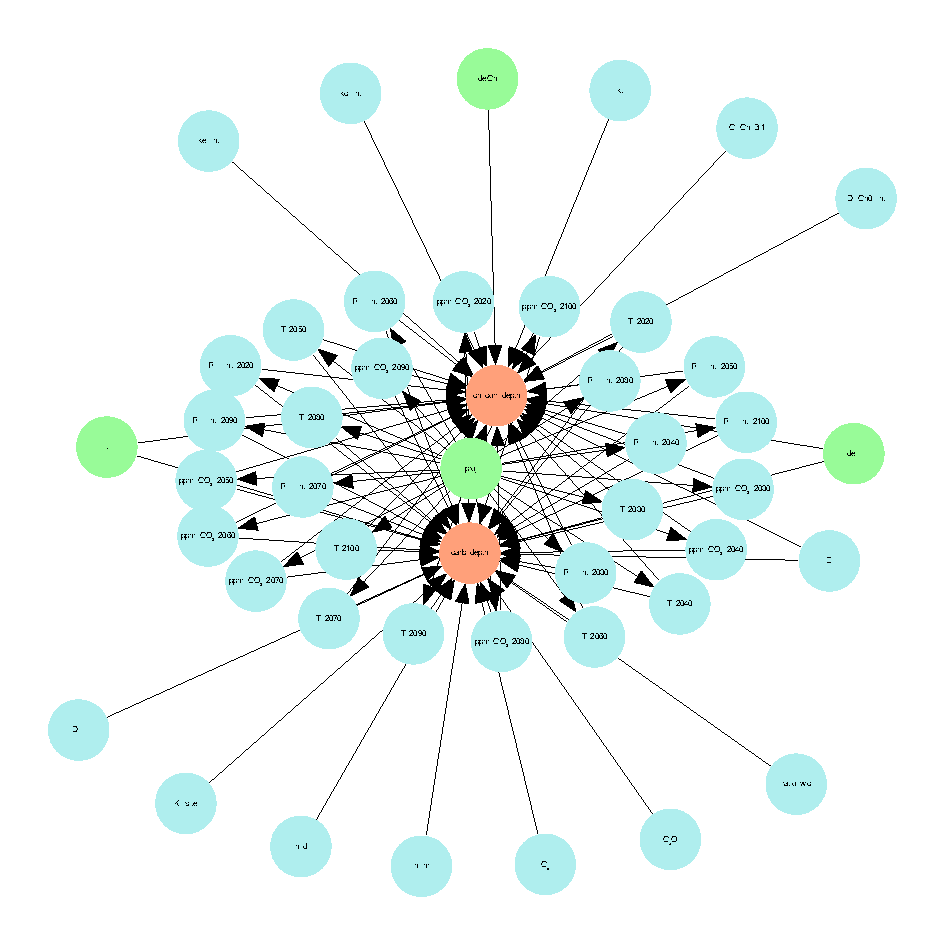
\includegraphics[width=\linewidth]{imgs/pdfs/12_total_ebn_precise.pdf}
    \caption{Carbonation and chloride induced corrosion phenomena eBN with precise nodes}\label{fig:precise_ebn}
\end{figure}

The functional nodes \textit{ch\_corr\_depth} and \textit{carb\_depth} are initially defined through the set of continuous random variables coming from their continuous parents, the set of discrete random variables coming from their discrete parents, and a simulation techinque, selected to be a standard Monte Carlo with $10^4$ samples for both of them. The union of these two sets of inputs together with the chosen simulation technique and two performance functions, one for the chloride induced corrosion and one for the carbonation model, allows to solve the structural reliability problems. In this way is possible to obtain the two CPTs associated with the two discrete nodes \textit{ch\_corr\_depth} and \textit{carb\_depth} in the reduced BN of Fig.~\ref{fig:precise_rbn}. 

\begin{figure}[H]
    \centering
    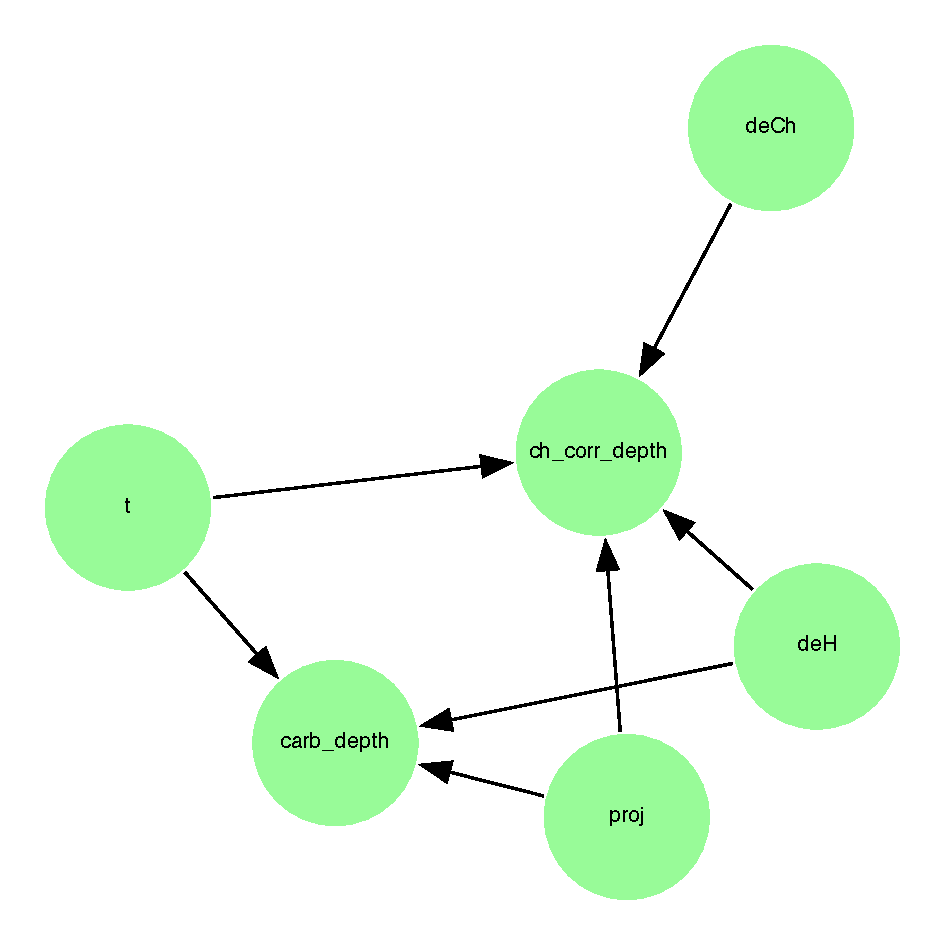
\includegraphics[width=\linewidth]{imgs/pdfs/13_total_rbn_precise.pdf}
    \caption{Carbonation and chloride induced corrosion phenomena reduce BN with precise nodes}\label{fig:precise_rbn}
\end{figure}

In this BN only discrete nodes are present. Both the evaluated nodes  \textit{ch\_corr\_depth} and \textit{carb\_depth} have as parents the discrete nodes refered to the specific time slice, to the specific climatic projection, and the auxiliary discrete node \textit{deH}. The node \textit{deCh} influences the sole node chloride induced corrosion process, therefore it is not a parent of \textit{carb\_depth}.

\begin{figure}[H]
    \centering
    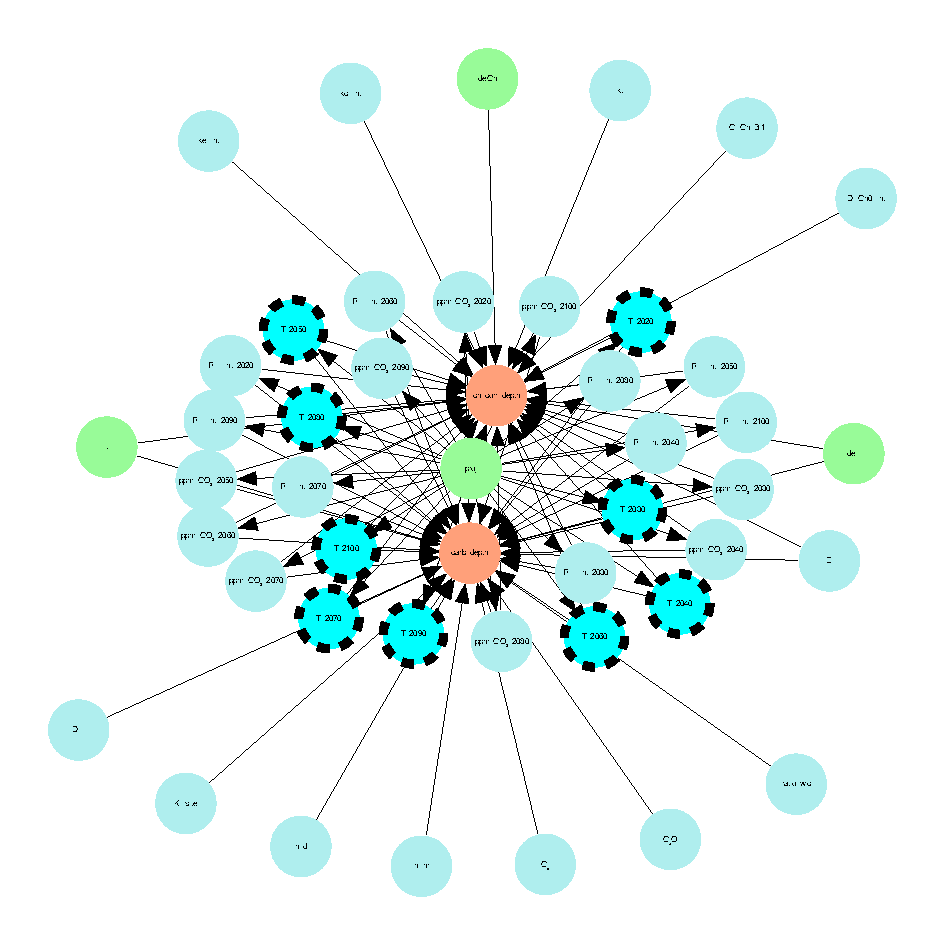
\includegraphics[width=\linewidth]{imgs/pdfs/14_total_ebn_imprecise.pdf}
    \caption{Carbonation and chloride induced corrosion phenomena eBN with imprecise temperature nodes}\label{fig:imprecise_ebn}
\end{figure}

In the climatic change catalogue~\cite{Copernicus_Climate_Change} data for each SSP come from different simulations. The guassian distributions defined in the tables Tab.~\ref{Climate_Change_Tnode_dists},~\ref{Climate_Change_RHnode_dists}, and~\ref{Climate_Change_CO2node_dists} have been hypotized by the author and their parameter have been extracted under this hypothesis to fit the dataset.
A more robust way for dealing with the epistemic uncertainty problem of future projections is represented by the interval probability theory. Therefore without introducing any specific hypothesis over the specific distribution the quantities of interest have treated as an interval defined only by an upper bound and a lower bound given respectively by the maximum and minimum value of all the simulations related to a specific SSP.\\
This concept has been applied to temperature projection obtaining the new node presented in Fig.~\ref{fig:imprecise_ebn} and defined in Tab.~\ref{Climate_Change_Tnode_interval}. The reduced BN of this imprecise eBN is the Credal Network presented in Fig.~\ref{fig:imprecise_rbn}.

\begin{figure}[H]
    \centering
    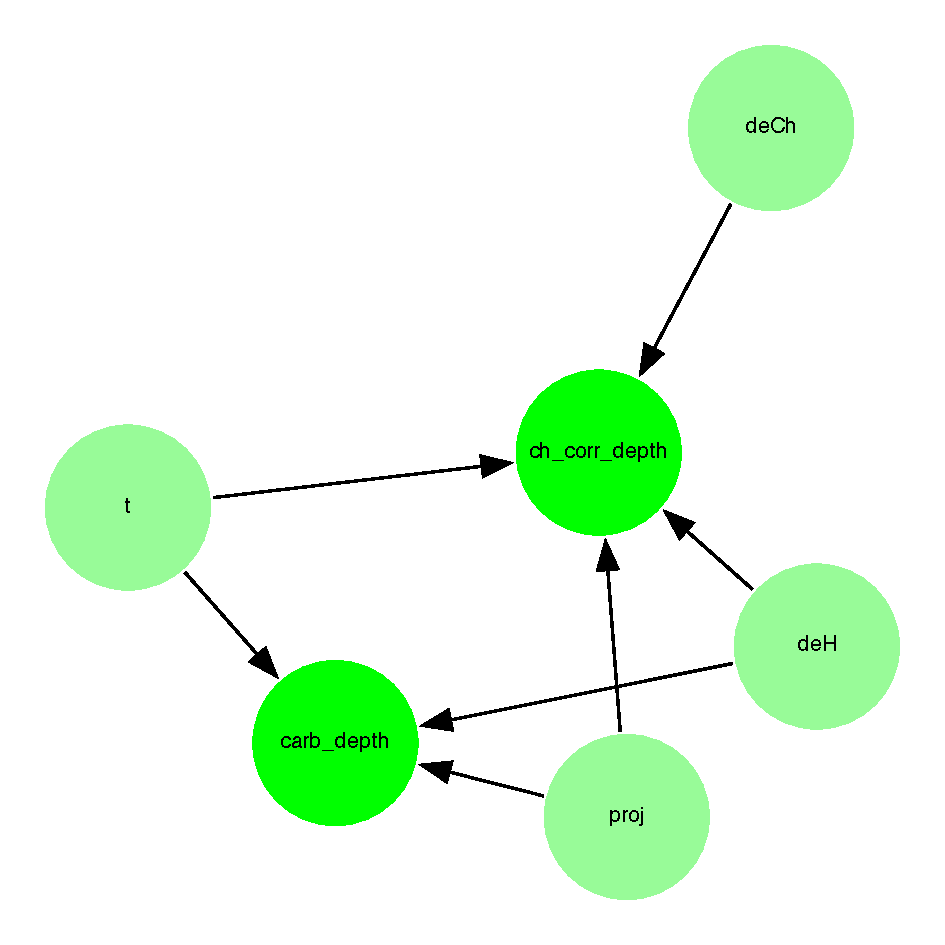
\includegraphics[width=\linewidth]{imgs/pdfs/15_total_rbn_imprecise.pdf}
    \caption{Carbonation and chloride induced corrosion phenomena reduce BN with imprecise nodes}\label{fig:imprecise_rbn}
\end{figure}

\begin{table}[H]
    \begin{center}
    \caption{Temperature nodes CPTs for the imprecise eBN of Fig.\ref{fig:imprecise_ebn}. Temperatures are measured in $K$}\label{Climate_Change_Tnode_interval}
        \begin{tabular}{P{2.5cm}P{7.7cm}}
            \toprule
            \textbf{Node} & \textbf{CPT} \\
            \midrule
            $T \_ 2020$ & 
                \begin{tabular}{P{2.4cm}P{2cm}P{2cm}}
                    \textbf{proj} & \textbf{lb} & \textbf{ub}\\
                    \midrule
                    \:ssp1 & $281.8723$ & $285.5608$\\ 
                    \:ssp2 & $281.6916$ & $286.8414$ \\
                    \:ssp5 & $281.5062$ & $286.7255$ \\
                \end{tabular}
            \\
            \midrule
            $T \_ 2030$ & 
                \begin{tabular}{P{2.4cm}P{2cm}P{2cm}}
                    \textbf{proj} & \textbf{lb} & \textbf{ub}\\
                    \midrule
                    \:ssp1 & $282.0982$ & $287.0741$ \\
                    \:ssp2 & $282.2602$ & $286.8415$ \\
                    \:ssp5 & $281.5062$ & $286.7255$ \\
                \end{tabular}
            \\
            \midrule
            $T \_ 2040$ & 
                \begin{tabular}{P{2.4cm}P{2cm}P{2cm}}
                    \textbf{proj} & \textbf{lb} & \textbf{ub}\\
                    \midrule
                    \:ssp1 & $282.2752$ & $285.7549$ \\
                    \:ssp2 & $282.2368$ & $287.6774$ \\
                    \:ssp5 & $281.8712$ & $287.1479$ \\
                \end{tabular}
            \\
            \midrule
            $T \_ 2050$ & 
                \begin{tabular}{P{2.4cm}P{2cm}P{2cm}}
                    \textbf{proj} & \textbf{lb} & \textbf{ub}\\
                    \midrule
                    \:ssp1 & $282.1972$ & $286.3009$ \\
                    \:ssp2 & $282.1169$ & $286.5602$ \\
                    \:ssp5 & $282.6306$ & $287.7634$ \\
                \end{tabular}
            \\
            \midrule
            $T \_ 2060$ & 
                \begin{tabular}{P{2.4cm}P{2cm}P{2cm}}
                    \textbf{proj} & \textbf{lb} & \textbf{ub}\\
                    \midrule
                    \:ssp1 & $281.9507$ & $287.6729$ \\
                    \:ssp2 & $282.8809$ & $287.8323$ \\
                    \:ssp5 & $284.1444$ & $288.1458$ \\
                \end{tabular}
            \\
            \midrule
            $T \_ 2070$ & 
                \begin{tabular}{P{2.4cm}P{2cm}P{2cm}}
                    \textbf{proj} & \textbf{lb} & \textbf{ub}\\
                    \midrule
                    \:ssp1 & $282.4679$ & $286.3140$ \\
                    \:ssp2 & $282.1799$ & $287.8909$ \\
                    \:ssp5 & $283.5394$ & $289.1019$ \\
                \end{tabular}
            \\
            \midrule
            $T \_ 2080$ & 
                \begin{tabular}{P{2.4cm}P{2cm}P{2cm}}
                    \textbf{proj} & \textbf{lb} & \textbf{ub}\\
                    \midrule
                    \:ssp1 & $282.0230$ & $287.2399$ \\
                    \:ssp2 & $283.1048$ & $287.3655$ \\
                    \:ssp5 & $284.8888$ & $289.7104$ \\
                \end{tabular}
            \\
            \midrule
            $T \_ 2090$ & 
                \begin{tabular}{P{2.4cm}P{2cm}P{2cm}}
                    \textbf{proj} & \textbf{lb} & \textbf{ub}\\
                    \midrule
                    \:ssp1 & $281.3064$ & $288.7765$ \\
                    \:ssp2 & $282.5490$ & $287.8518$ \\
                    \:ssp5 & $284.3658$ & $290.5262$ \\
                \end{tabular}
            \\
            \midrule
            $T \_ 2100$ & 
                \begin{tabular}{P{2.4cm}P{2cm}P{2cm}}
                    \textbf{proj} & \textbf{lb} & \textbf{ub}\\
                    \midrule
                    \:ssp1 & $281.7551$ & $287.4349$ \\
                    \:ssp2 & $283.0796$ & $288.4324$ \\
                    \:ssp5 & $285.1481$ & $292.2743$ \\
                \end{tabular}
        \end{tabular}
    \end{center}
\end{table}

